
\subsection{Snort-Konfiguration}

Die Hauptkonfigurationsdatei für snort liegt unter \inlinecodee{/etc/snort/snort.conf}. In diesem Fall muss allerdings zuerst die Debian-spezifische Datei \inlinecodee{/etc/snort/snort.debian.conf} entsprechend Abb. \ref{fig:snort-debian-conf} bearbeitet werden. Das Feld \inlinecodee{DEBIAN\_SNORT\_INTERFACE} wird entsprechend Abschnitt \ref{sec:ip-dist} gesetzt.

\begin{figure}[H]
\centering
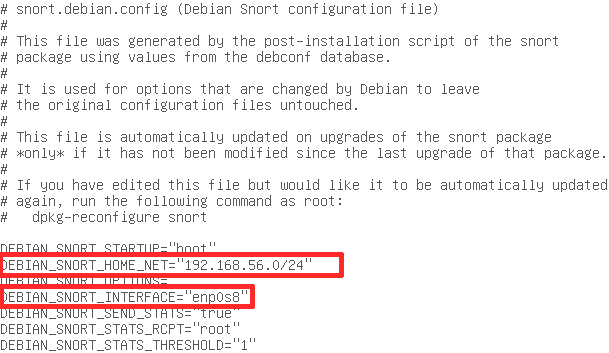
\includegraphics[width=0.6\textwidth]{graphics/attacks/snort-debian.png}
\caption{\inlinecodee{/etc/snort/snort.debian.conf}}\label{fig:snort-debian-conf}
\end{figure}


Es gibt einige vorgefertigte Regeln, welche unter \inlinecodee{/etc/snort/rules} zu finden sind.
In \inlinecodee{/etc/snort/snort.conf} findet man am Ende der Datei alle Regeln (Pfade), die snort einbeziehen soll, d.h die Regeln, die tatsächlich aktiv sind.

Um die Konfiguration nach dem Bearbeiten auf Fehler zu prüfen, kann man folgenden Befehl nutzen.
\begin{minted}{bash}
  /sbin/snort -T -i enp0s8 -c /etc/snort/snort.conf
\end{minted}

\notebo{Info}{
Snort kann über die Tastenkombinaition \inlinecodee{Ctrl+z} beendet werden.
}


\subsection{Benutzerdefinierte Regeln}

Die Regeldefinitionen folgen einer einfachen Syntax. Die grundlegende Struktur zeigt Abb. \ref{fig:snort-rule-syntax}. Als Referenz eignen sich auch die vorgefertigten Regeln unter \inlinecodee{/etc/snort/rules}.

\begin{figure}[H]
\centering
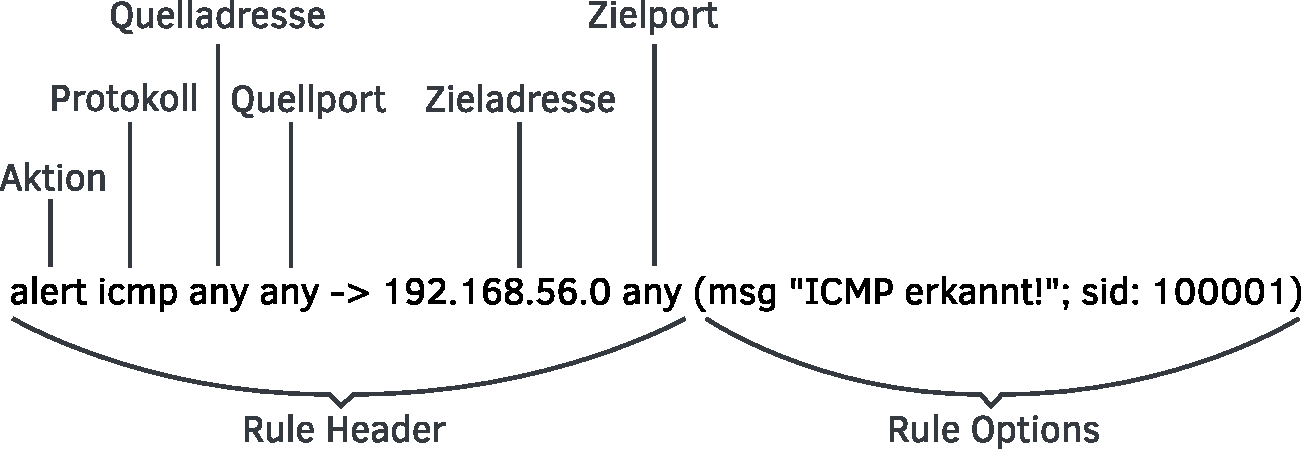
\includegraphics[width=0.6\textwidth]{graphics/attacks/rule-syntax.pdf}
\caption{Struktur der Snort-Regeln.}\label{fig:snort-rule-syntax}
\end{figure}

Die dargestellte Regel alarmiert bei Erkennung eines ICMP-Paketes (z.B. ping). Um sie hinzuzufügen fügt man die Zeile aus Abb \ref{fig:snort-rule-syntax} in die zuerst leere Datei \inlinecodee{/etc/snort/rules/local.rules} ein. Die Zieladresse kann auch durch die Umgebungsvariable \inlinecodee{\$HOME\_{NET}} ersetzt werden (Abb. \ref{fig:snort-localrules1}). \footnote{Die \inlinecodee{sid} kann quasi ein beliebiger einzigartiger Wert sein.}\\

\begin{figure}[H]
\centering
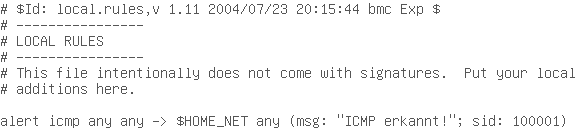
\includegraphics[width=0.6\textwidth]{graphics/attacks/localrules1.png}
\caption{\inlinecodee{/etc/snort/rules/local.rules}}\label{fig:snort-localrules1}
\end{figure}


Dann startet man snort mit dem Befehl
\begin{minted}{bash}
  /sbin/snort -q -l /var/log/snort -i enp0s8 -A console -c /etc/snort/snort.conf
\end{minted}

Danach kann vom Angreifer ein \inlinecodee{ping}-Befehl auf den Victim-Host durchgeführt werden, welcher wie in Abb. \ref{fig:snort-ping} durch snort erkannt werden sollte.

\begin{figure}[H]
  \centering
  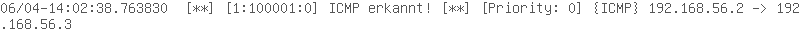
\includegraphics[width=0.8\textwidth]{graphics/attacks/snort-ping.png}
  \caption{Ergebnis des Ping-Tests.}\label{fig:snort-ping}
\end{figure}

Als Hilfe zur Erstellung von Regeln eignet sich die Website \textit{snorpy} \cite{snorpy}, welche eine grafische Oberfläche bietet, um Regeln zu erstellen und mögliche Optionen zu erkunden.

\subsection{nmap}
Mit der Standardkonfiguration lässt sich ein einfacher \inlinecodee{nmap}-Scan sofort erkennen.\\
Vom Angreifer aus:
\begin{minted}{bash}
  nmap 192.168.56.3
\end{minted}

\begin{figure}[H]
  \centering
  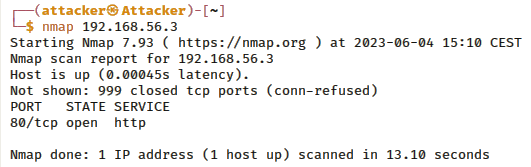
\includegraphics[width=0.5\textwidth]{graphics/attacks/nmap-kali-working.png}
  \caption{Ergebnis von nmap beim Angreifer.}\label{fig:nmap2}
\end{figure}

Das Resultat des NIDS zeigt Abb. \ref{fig:nmap1}.

\begin{figure}[H]
  \centering
  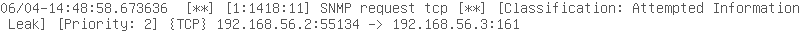
\includegraphics[width=0.8\textwidth]{graphics/attacks/nmap.png}
  \caption{NIDS altert bei nmap.}\label{fig:nmap1}
\end{figure}

\subsection{DoS-Angriff / SYN-Flood}\label{sec:dos}

Die Standardkonfiguration von snort kann bereits DoS-Angriffe erkennen. Für eine einfache benutzerdefinierte Konfiguration kann man die folgende Regel verwenden.

\begin{minted}{bash}
  alert tcp any -> $HOME_NET 80 (flag: S; msg: "Potentieller DoS-Angriff!"; sid: 100002)
\end{minted}

Hierbei wird die Option \inlinecodee{flag: S} genutzt, um TCP-Pakete zu erkennen, bei denen nur das SYN-Flag gesetzt ist. Weitere Flags finden sich in der snort-Dokumentation \cite{snortflag}.\\

Der Webserver auf dem Victim-Host sollte bereits mit einer Beispielseite laufen. Dies kann z.B. über Firefox auf dem Angreifer überprüft werden. Da der Webbrowser aufgrund von Caching ungeeignet ist für die Erkennung des Serverzustandes, kann man alternativ den folgenden Befehl nutzen.

\begin{minted}{bash}
  curl -I 192.168.56.3
\end{minted}

Dieser sollte bei erfolgreicher Bearbeitung durch den Server die in Abb. \ref{fig:nginx-1} zu sehende Ausgabe liefern.\\

\begin{figure}[H]
\centering
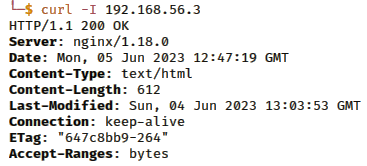
\includegraphics[width=0.4\textwidth]{graphics/attacks/curl-result1.png}
\caption{Erfolgreiche Webserverantwort.}\label{fig:nginx-1}
\end{figure}

Das auf Kali vorinstallierte Tool \inlinecodee{hping3} kann nun für einen einfachen TCP SYN-Angriff verwendet werden. Dazu wird folgender Befehl genutzt.\\

\begin{minted}{bash}
  sudo hping3 --flood -S --rand-source -p 80 192.168.56.3
\end{minted}

Nun kann die Seite erneut angefragt werden (z.B. auf dem Angreifer-System). Es sollte zu Verzögerungen kommen. Gleichzeitig sollte das snort-System die Anfragen als \glqq{}Potentially Bad Traffic\grqq{} klassifizieren (Abb. \ref{fig:dos-snort}). Als Variation kann man das Argument \inlinecodee{--rand-source} im \inlinecodee{hping3} weglassen.
Sind keine Verzögerungen merkbar, kann der folgende alternative Befehl zu Anfrage möglicherweise helfen.
\begin{minted}{bash}
  curl -I 192.168.56.3 -H "Cache-Control: no cache"
\end{minted}

\begin{figure}[H]
\centering
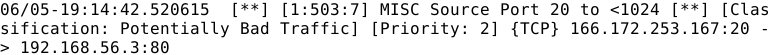
\includegraphics[width=0.6\textwidth]{graphics/attacks/snort-dos.png}
\caption{SYN-Angriffserkennung durch snort.}\label{fig:dos-snort}
\end{figure}
